\documentclass[a4paper,12pt]{article} % добавить leqno в [] для нумерации слева
\usepackage[a4paper,top=1.3cm,bottom=2cm,left=1.5cm,right=1.5cm,marginparwidth=0.75cm]{geometry}
%%% Работа с русским языком
\usepackage{cmap}					% поиск в PDF
\usepackage{mathtext} 				% русские буквы в фомулах
\usepackage[T2A]{fontenc}			% кодировка
\usepackage[utf8]{inputenc}			% кодировка исходного текста
\usepackage[english,russian]{babel}	% локализация и переносы

\usepackage{graphicx}
\usepackage{mathtools}
\usepackage{wrapfig}
\usepackage{tabularx}
\usepackage{amssymb}
\usepackage{hyperref}
\usepackage[rgb]{xcolor}
\hypersetup{colorlinks=true,urlcolor=blue}
%% Шрифты
\usepackage{euscript}	 % Шрифт Евклид
\usepackage{amsmath}
\usepackage{mathtools}
%%% Заголовок
\author{Lokhmatov Arseniy}
\title{Лабораторная работа по общей физике}

\date{\today}
\begin{document}
\begin{titlepage}
    \newpage
    \begin{center}
    {\large МОСКОВСКИЙ ФИЗИКО-ТЕХНИЧЕСКИЙ ИНСТИТУТ (НАЦИОНАЛЬНЫЙ ИССЛЕДОВАТЕЛЬСКИЙ УНИВЕРСИТЕТ)}
    \vspace{1cm}

    {\largeФизтех-школа аэрокосмических технологий}
    \vspace{6em}
    \end{center}
    
    \vspace{1.2em}

    \begin{center}
    %\textsc{\textbf{}}
    \Large Лабораторная работа №3.2.5 \\
    Свободные и вынужденные колебания в электрическом контуре
    \linebreak
    \end{center}
    
    \vspace{11em}
    
    \begin{flushright}
                       {\large Работу выполнил\\
                       Лохматов Арсений Игоревич\\
                       Козярский Алексей Сергеевич\\
                       Б03-303 }
    \end{flushright}

    \vspace{\fill}

    \begin{center}
        
\includegraphics[width=0.2\linewidth]{dasr.png}
    \end{center}

    \begin{center}
    Долгопрудный, 2024
    \end{center}

    \end{titlepage}

\section{Теоретическая часть}

\paragraph{Цель работы:} исследование свободных и вынужденных колебаний в колебательном контуре.

\paragraph{Оборудование:} осциллограф АКТАКОМ ADS-6142H, генератор сигналов специальной формы АКИП-3409/4, магазин сопротивления МСР-60, магазин емкости Р5025, магазин индуктивности Р567 типа МИСП, соединительная коробка с шунтирующей емкостью, соединительные одножильные и коаксиальные провода.

\subsection{Экспериментальная установка}

Схема установки для исследования колебаний приведена на рисунке 1.\par\par

\begin{figure}[h]
\begin{center}
		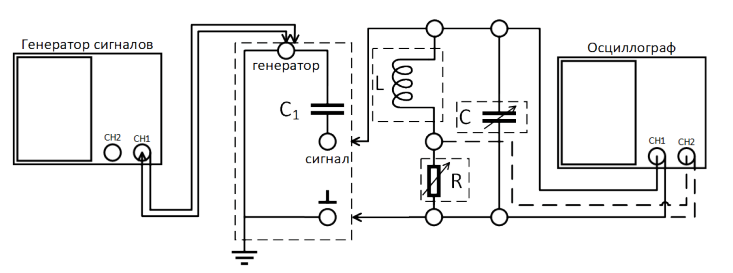
\includegraphics[width=15cm]{image_1.png}
\end{center}
	\caption{\textit{Схема установки для исследования вынужденных колебаний}}
	\label{img1}
\end{figure}

Колебательный контур состоит из постоянной индуктивности $L$ с активным сопротивлением $R_L$, переменной емкости $C$ и сопротивления $R$. Картина колебаний напряжения на емкости наблюдается на экране осциллографа. Для возбуждения затухающих колебаний используется генератор сигналов. Сигнал с генератора поступает через конденсатор $C_1$ на вход колебательного контура. Данная емкость необходима чтобы выходной импеданс (сопротивление) генератора был много меньше импеданса колебательного контура и не влиял на процессы, проходящие в контуре.\par

При изучении свободно затухающих колебаний генератор специальных сигналов на вход колебательного контура подает периодические короткие импульсы, которые заряжают конденсатор $C$. За время между последовательными импульсами происходит разрядка конденсатора через резистор и катушку индуктивности. Напряжение на конденсаторе $U_C$ поступает на вход канала $1(X)$ электронного осциллографа. Для наблюдения фазовой картины затухающих колебаний на канал $2(Y)$ подается напряжение с резистора $R$ (пунктирная линия на схеме установки), которое пропорционально току $I$ $(I \sim \frac{dU_C}{dt})$.\par

При изучении возбужденных колебаний на вход колебательного контура подается
синусоидальный сигнал. С помощью осциллографа возможно измерить зависимость
амплитуды возбужденных колебаний в зависимости от частоты внешнего сигнала,
из которого возможно определить добротность колебательного контура. Альтернативным способом расчета добротности контура является определение декремента затухания по картине установления возбужденных колебаний. В этом случае генератор сигналов используется для подачи цугов синусоидальной формы.

\section{Практическая часть}

В работе предлагается исследовать параллельный колебательный контур несколькими способами:

\begin{enumerate}
    \item Изучение свободных колебаний в электрическом контуре;
    \begin{enumerate}
        \item Определение зависимости периода свободных колебаний контура от емкости;
        \item Определение зависимости логарифмического декремента затухания от сопротивления;
        \item Определение критического сопротивления контура;
    \end{enumerate}
    \item Изучение вынужденных колебаний в электрическом контуре;
    \begin{enumerate}
        \item Построение резонансных кривых колебательного контура: АЧХ и ФЧХ;
        \item Изучение процесса установления и затуханий колебаний;
        \item Определение декремента затухания колебательного контура по нарастанию колебаний и по их затуханию;
    \end{enumerate}
    \item Определение добротности контура различными способами.
\end{enumerate}

\subsection{Подготовка приборов к работе}

\begin{enumerate}
    \item Подключили генератор специальных сигналов к входу $1(X)$ осциллографа;
    \item Установили на генераторепоследовательность импульсов, выставили длительность импульсов $10 мкс$, частоту повторения импульсов $100 Гц$, амплитуду сигнала $20 В$. Подали сигнал на осциллограф;
    \item Получили на осциллографе статическое изображение периодических сигналов;
    \item Собрали электрическую схему согласно рис. \ref{img1}.
\end{enumerate}

\subsection{Измерение периодов свободных колебаний}

\begin{enumerate}
    \item Установили на магазине сопротивлений величину $R = 0 Ом$, на магазине индуктивностей $L = 100 мГн$, на магазине ёмкостей величину $C = 0 мкФ$. Не смотря на это контур сам по себе обладает некоторым минимальным значением ёмкости $C_0$, благодаря которому в контуре реализуются свободные колебания. При этом затухание обеспечивается наличием активного сопротивления в магазине индуктивностей $R_L$. Получили на экране осциллографа картину свободных затухающих колебаний.
    \item Подобрали частоту развёртки осциллографа, при которой расстояние между импульсами генератора занимает почти весь экран;
    \item Измерили с помощью осциллографа период затухающих колебаний. 
    
    \[ T_{\text{затух}} = 66 \text{мс} \]

    \item По периоду колебаний определили нулевую ёмкость колебательного контура. Это значение является минимальным для магазина ёмкостей и его необходимо учитывать при дальнеших расчётах.

    \[ T_0 = 2\pi \sqrt{LC_0} \longrightarrow C_0 = \frac{T^2}{4\pi^2L} \approx 0.0011 \text{мкФ} \]

    \item Изменяем ёмкость проведём измерения периодов. Результаты занесём в таблицу \ref{table1}. Так же рассчитаем теоретические значения периодов по формуле Томсона и построим график $T_{\text{exp}} = f(T_{\text{theor}})$.

    \end{enumerate}

    \begin{table}[h]
		\centering
		\begin{tabular}{|c|c|c|c|}
		\hline
		$C + C_0$, мкФ & $T_{exp}$, мкс & $T_{th}$, мкс & \tau, \% \\ \hline
            0.0011 & 66 & 65.9 & 0.15 \\
		  0.0021 & 91 & 91.1 & 0.06 \\
		  0.0031 & 110 & 110.6 & 0.57 \\
		0.0041 & 127 & 127.2 & 0.18 \\
		0.0051 & 143 & 141.9 & 0.77 \\
		0.0061 & 156 & 155.2 & 0.52 \\
            0.0071 & 168 & 167.4 & 0.34 \\
            0.0081 & 179 & 178.8 & 0.1 \\
		\hline
		\end{tabular}
		\caption{Экспериментальные и теоретические значения периодов колебаний}
            \label{table1}
    \end{table}

    \begin{figure}[h]
    \begin{center}
		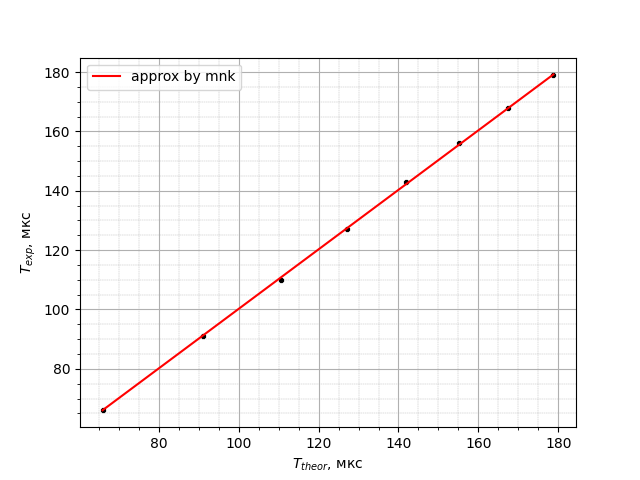
\includegraphics[width=15cm]{plot_1.png}
    \end{center}
	\caption{\textit{Теоретические и экспериментальные значения периодов исследуемых колебаний}}
	\label{plot1}
    \end{figure}
    
    В последнем столбце рассчитаем отклонение экспериментального значения от теоретического по формуле $\tau = \frac{\left| T_{th} - T_{exp} \right|}{T_{th}} \cdot 100 \%$. Отклонение получилось очень маленькое, что говорит о высокой точности измерений. Метод наименьших квадратов аппроксимирует наш график, погрешность определения угла наклона составляет $\sigma_\alpha = 0.139 \%$.

    \[ \alpha = 1.002217 \pm 0.001387 \]

\newpage

\subsection{Критическое сопротивление и декремент затухания}

\begin{enumerate}
    \item Приняв $L = 100 \text{мГн}$, рассчитаем емкость $C^*$, при которой собственная частота колебаний $\nu_0 = \frac{1}{2\pi \sqrt{LC^*}}$ составляет $6.5 \text{кГц}$. 
    
    \[ \nu_0 = \frac{1}{2\pi \sqrt{LC^*}} \Longleftrightarrow C^* = \frac{1}{(4\pi^2L\nu_{0})} = \frac{1}{(4\pi^2\cdot100\cdot10^{-3}\cdot6.5^2\cdot10^6)} \approx 5.995 \text{нФ} \]
    
    Для выбранных $L$ и $C^*$ рассчитаем критическое сопротивление контура $R_{\text{cr}}$ по формуле:
    \[ R_{\text{cr}} = 2\sqrt{\frac{L}{C^*}} = 2 \cdot \sqrt{\frac{100 \cdot 10^{-3}}{5.995 \cdot 10^{-9}}} \approx 8168.4 \text{Ом}. \]

    \item Установим на магазине емкость, близкую к рассчитанной критической и запишите ее значение:
    
    \[ C_{\text{now}} = 6 \text{нФ}. \]
    
    Увеличивая сопротивление $R$ от нуля до $R_{\text{cr}}$, наблюдаем картину затухающих колебаний на экране осциллографа. Определим сопротивление магазина, при котором колебательный режим переходит в апериодический.
    \[ R_{\text{aper}} = 5500 \text{Ом}. \]

    \item Установим сопротивление $(0.05 - 0.25) \cdot R_{cr}$. Получим на экране картину затухающих колебаний. Для расчета логарифмического декремента затухания $\Theta$ измерим амплитуды, разделенные целым числом периодов $n$, воспользуемся формулой:

    \[ \Theta = \frac{1}{n} \cdot \ln{\frac{U_{m}}{U_{m+n}}} = \ln{\frac{U_{m}}{U_{m+1}}}, \text{при } n = 1. \]

\end{enumerate}

    \begin{table}[h]
		\centering
		\begin{tabular}{|c|c|c|c|c|}
			\hline
			$R_{\text{вн}}$, Ом & $R = R_{\text{вн}} + R_L$, Ом& $\theta = \ln \frac{U_k}{U_{k+1}}$ & $Q = \frac{\pi}{\theta}$ & $\sigma_{Q}$ \\ \hline
			 204 ($0,025R_{cr}$) & 204 + 43 = 247 & 0.210 & 14.959 & 0.299 \\ \hline
		408 ($0,05R_{cr}$) & 408 + 43 = 451 & 0.386 & 8.139 & 0.163  \\ \hline
			816 ($0,1R_{cr}$) & 816 + 43 = 854 & 0.684 & 4.593 & 0.092 \\ \hline
			 2042 ($0,25R_{cr}$) & 2042 + 43 = 2085 & 1.123 & 2.798 & 0.056 \\ \hline
		\end{tabular}
		\caption{Декремент затухания свободных колебаний}
	\end{table}

    Погрешность определения декремента затухания состоит из погрешности определения напряжения. Мы пользовались цифровым осциллографом $АКТАКОМ ADS-6142H$, в паспорте которого указано принять систематическую ошибку $\sim 2 \%$.

    Построим график зависимости $\frac{1}{\theta^2} = f(\frac{1}{R^2})$. Так как
	\[\theta = \ln\left(\frac{U_k}{U_{k + 1}}\right) = \gamma T = \gamma \frac{2\pi}{\omega_1} \Longleftrightarrow \theta^2 = \gamma^2\frac{4\pi^2}{\omega_1^2} = \gamma^2 \frac{4\pi^2}{\omega_0^2 - \gamma^2} \Longleftrightarrow \]
	\[ \Longleftrightarrow \frac{1}{\theta^2} = \frac{1}{4\pi^2}\cdot\left(\frac{\omega_0^2}{\gamma^2} - 1\right) = \frac{1}{4\pi^2}\cdot\left(\frac{4L}{CR^2} - 1\right)\]
	
	то зависимость должна получиться линейной:
	
	\[\frac{1}{\theta^2} = \frac{1}{R^2}\cdot\frac{L}{C\pi^2} - \frac{1}{4\pi^2}.\]

     Запишем общий вид линейной функции:

        \[ y = a \cdot x + b, \]

    если принять обозначения $x = \frac{1}{R^2}$ и  $y = \frac{1}{\theta^2}$, то получим, что $a = \frac{L}{C\pi^2}$ - угловой коэффициент функции, $b = - \frac{1}{4\pi^2}$ - сдвиг по оси ординат.

    \begin{figure}[h]
    \begin{center}
		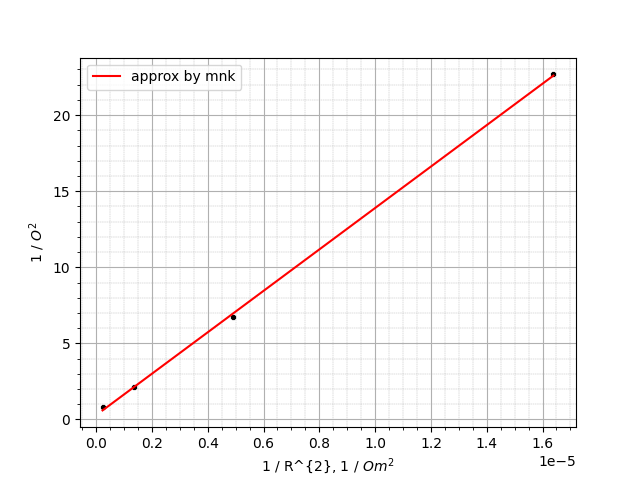
\includegraphics[width=15cm]{plot_3.png}
    \end{center}
	\caption{\textit{Зависимость декремента затухания от суммарного сопротивления}}
	\label{plot3}
    \end{figure}

    Аппроксимацию проводили с помощью метода наименьших квадратов, получили:
    \[ a = (136.151 \pm 1.875) \cdot 10^{4} Om^{2};\]
    \[ b = 0.282 \pm 0.161. \]

    Рассчитаем $R_{cr}^{lab}$ по формуле:
    \[ R_{cr}^{lab} = 2\pi\sqrt{\frac{\Delta x}{\Delta y}} = 2\pi\sqrt{a} = 2\pi\sqrt{136.151 \cdot 10^{4}} = 7331.457 \pm 860.361 Om.  \]

    Видим, что с учётом погрешности, высчитанной с помощью метода наименьших квадратов, полученное значение совпадает с рассчитанным ранее теоретическим $R_{cr}$.

\newpage

\subsection{Свободные колебания на фазовой плоскости}

\begin{enumerate}
    \item  Введём сопротивление $R \approx 0.05 \cdot R_{cr} \approx 408 Om$ на магазине. Подадим на канал 2(Y) осциллографа падение напряжения с резистора.

    \item Для одновременного наблюдения осциллограмм тока и напряжения свободных затухающих колебаний переведём осциллограф в двухканальный режим. Подберём масштабы по вертикали и частоту развертки по горизонтали так, чтобы оба сигнала были представлены на временном интервале, слегка превышающем период повторения импульсов с генератора.

    \item Подберём частоту повторения импульсов на генераторе так, чтобы расстояние между импульсами было порядка характерного времени затухания свободных колебаний (эта частота составляет 400-500 Гц, у нас получилось 450).

    \item Для наблюдения затухающих колебаний на фазовой плоскости отключим развертку по времени. Меняя чувствительность каналов, подберём масштаб спирали, удобный для измерений. Зарегистрируем спираль. 
    
    При том же значении $C_{now}$, что и в секции 2.3, наблюдайте за изменением спирали при увеличении сопротивления $(0.05 - 0.25) \cdot R_{cr}$.
    Для определения декремента затухания $\Theta$ измерим координаты пересечения
    витков спирали с одной из осью координат, разделенные целым числом периодов n, для значений сопротивлений, выбранных в секции 2.3.

    \begin{table}[h]
		\centering
		\begin{tabular}{|c|c|c|c|c|c|c|}
			\hline
			R, Ом & n & $U_k$, дел & $U_{k + n}$, дел & $\theta$ & $Q$ & $\sigma_{Q}$  \\ \hline
			408 & 5 & 18 & 4 & 0.301 & 10.44 & 0.731 \\ \hline
			2042 & 2 & 10 & 1 & 1.151 & 2.73 & 0.191 \\ \hline 
		\end{tabular}
		\caption{Определение добротности на фазовой плоскости}
	\end{table}

    Поскольку количество делений фиксировали мы, а не прибор, то относительную погрешность погрешность определения добротности можем принять равной $\epsilon_{Q} = 0.07$.

\end{enumerate}

\newpage

\subsection{Исследование резонансных кривых}

\begin{enumerate}
    \item Для наблюдения вынужденных колебаний переведём осциллограф в одноканальный режим просмотра (выключить режим $XY$). 

    \item Переведём генератор специальных сигналов в режим подачи синусоидального сигнала.

    \item Выставим значение емкости $C^{*}$ из секции 2.3, а сопротивление R1 из значений зафиксированных в секции 2.3.

    \begin{figure}[h]
    \begin{center}
		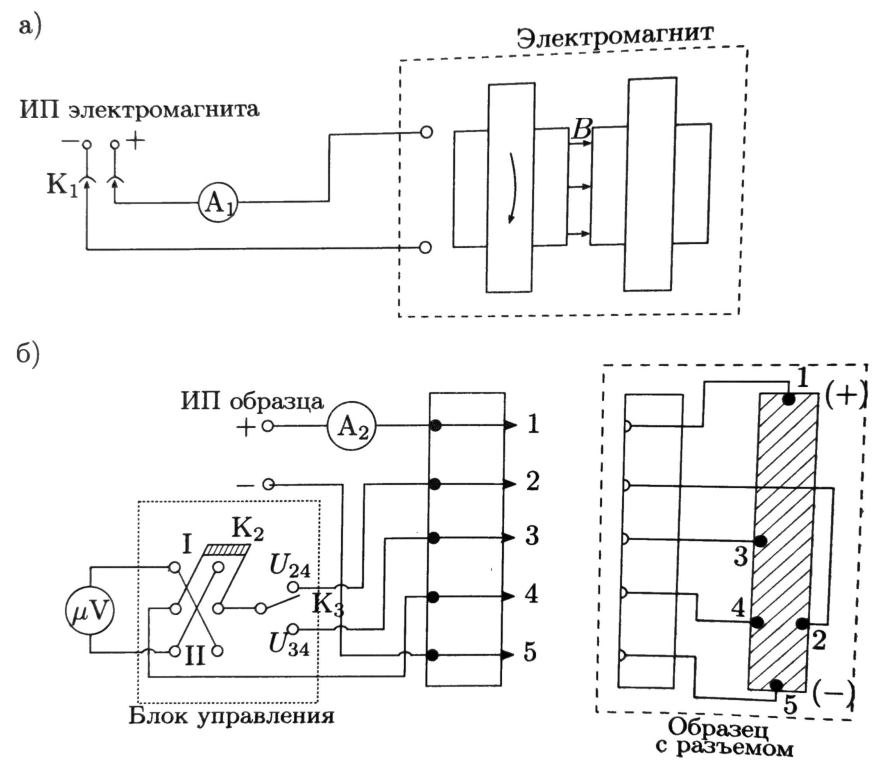
\includegraphics[width=15cm]{image_2.png}
    \end{center}
	\caption{\textit{Схема установки для исследования АЧХ и ФЧХ}}
	\label{image2}
    \end{figure}

    \item  С помощью переходника и коаксиальных кабелей подайте сигнал с генератора одновременно на колебательный контур и на канал 2 осциллографа (см. рисунок \ref{image2}). Добейтесь того чтобы на экране осциллографа можно было наблюдать одновременно два сигнала: сигнал, взятый с колебательного контура, на первом канале и первоначальный сигнал на втором канале.

    \item Убедились, что на экране осциллографа при частотах близких к резонансным наблюдается устойчивый синусоидальный сигнал.

    \item Изменяя частоту генератора вблизи резонансной частоты и наблюдая синусоиду на первом канале на экране осциллографа, убедились, что амплитуда колебаний максимальна при достижении резонансной частоты. Определите ее значение:

    \[ \nu^{1}_{res} = 6610 \text{Гц}. \]

    \item Снимем АЧХ и ФЧХ колебательного контура вблизи резонанса.

    \[ \Delta \phi = 2\pi \cdot \nu \cdot \Delta x \]

    \begin{table}[h]
		\centering
		\begin{tabular}{|c|c|c|c|}
			\hline
			$\nu$, Гц & $U$, В & $\Delta x$, мкс & $\Delta \phi$, $\cdot \pi$ \\ \hline
			6980.0 & 9.2 & 15.2 & 0.976 \\ \hline
                6932.6 & 9.6 & 15.6 & 1.038 \\ \hline
                6885.3 & 10.4 & 18.4 & 1.318 \\ \hline
                6837.9 & 10.6 & 20.0 & 1.45 \\ \hline
                6790.5 & 11.0 & 21.6 & 1.613 \\ \hline
                6743.1 & 11.4 & 24.8 & 1.906 \\ \hline
                6695.8 & 11.8 & 27.2 & 2.149 \\ \hline
                6648.4 & 12.4 & 29.6 & 2.44 \\ \hline
                6610.0 & 13.2 & 32.4 & 2.827 \\ \hline
		\end{tabular}
		\hspace{.06\textwidth}
		\begin{tabular}{|c|c|c|c|}
			\hline
			$\nu$, Гц & $U$, В & $\Delta x$, мкс & $\Delta \phi$, $\cdot \pi$ \\ \hline
			6553.6 & 12.8 & 36.4 & 3.053 \\ \hline
                6506.3 & 12.6 & 40.0 & 3.279 \\ \hline
                6458.9 & 11.4 & 42.8 & 3.151 \\ \hline
                6411.5 & 11.0 & 46.0 & 3.244 \\ \hline
                6364.1 & 10.2 & 49.2 & 3.194 \\ \hline
                6316.8 & 9.4 & 51.6 & 3.064 \\ \hline
                6269.4 & 9.0 & 55.2 & 3.115 \\ \hline
                6225.4 & 8.2 & 57.2 & 2.92 \\ \hline
		\end{tabular}
		\caption{АЧХ и ФЧХ для $R_1 = 451$ Ом}
		
	\end{table}

    \textbf{АЧХ:}

    Построим график по данным из таблицы в координатах  $ y = \frac{U}{U_{0}}, x = \frac{\nu}{\nu_0}$. 
    
    Определим добротность по графику. $Q = \frac{\omega_0}{2\Delta \Omega}$, где $2\Delta \Omega$ - ширина резонансной кривой на уровне $U = \frac{U_0}{\sqrt{2}}$.

    \[ \Longrightarrow 2\Delta \Omega = 0.0999 \Longrightarrow Q = \frac{0.98}{0.099} = 9.81 \]

    \textbf{ФЧХ:}

    Построим график по данным из таблицы в координатах  $ y = \phi, x = \frac{\nu}{\nu_0}$. 


    Проведем горизонтальную линию через уровень, где наблюдается резонанс ($\approx\frac{\pi}{2}$). Затем отразим одну половину относительно этой прямой и измерим приблизительно ширину на расстоянии $\frac{\pi}{4}$ от резонанса. Тогда:

    \[ \Longrightarrow Q = \frac{1.35}{0.07\cdot \pi} = 6.139. \]
    
\end{enumerate}

\begin{figure}[h]
    \begin{center}
		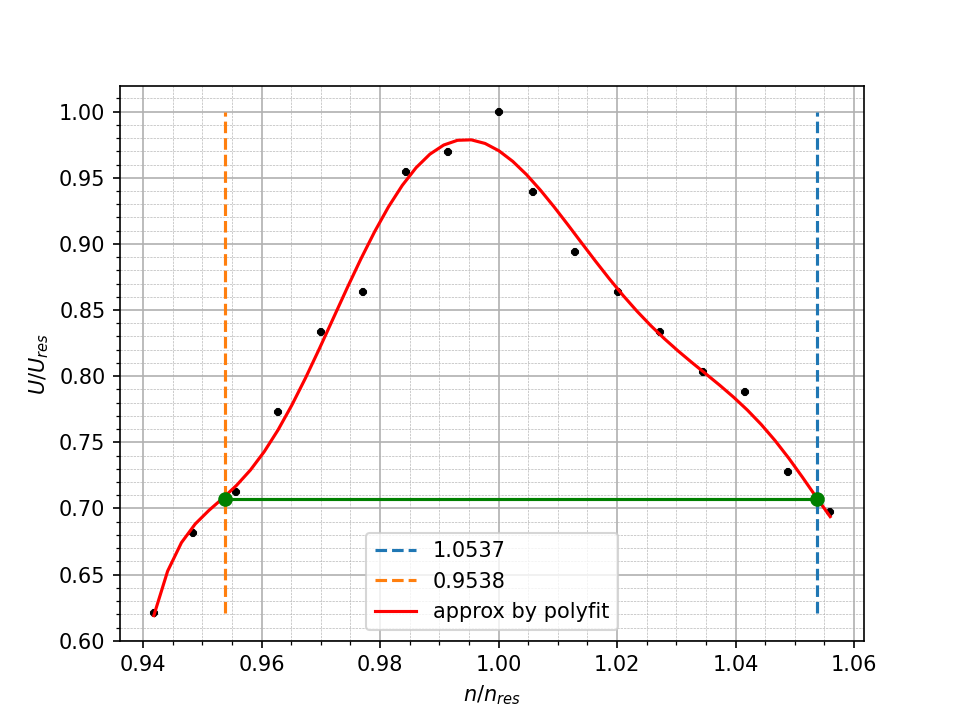
\includegraphics[width=14cm]{plot_4.png}
    \end{center}
	\caption{АЧХ при R = 451 Ом}
	\label{plot4}
    \end{figure}

\begin{figure}[h]
    \begin{center}
		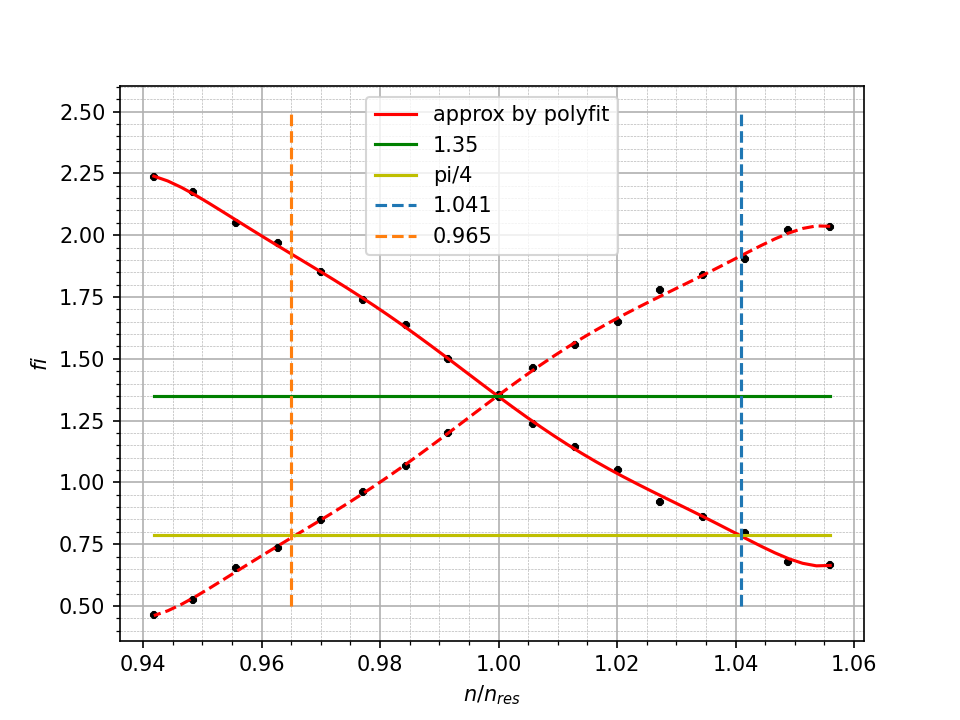
\includegraphics[width=14cm]{plot_5.png}
    \end{center}
	\caption{ФЧХ при R = 451 Ом}
	\label{plot5}
    \end{figure}

\newpage

\subsection{Определение теоретического значения добротности}

    Рассчитаем теоретическое значение добротности через параметры контура $L$, $C$ и $R$.

    \[ \theta = \ln{\frac{A(t)}{A(t+T)}} = \ln{\frac{A_0e^{-\beta t}}{A_0e^{-\beta(t+T)}}} = \ln{e^{\beta T}} = \beta T; \]

    \[Q = \frac{\pi}{\theta} = \frac{\pi}{\beta T} = \frac{\pi}{\frac{R}{2L}\frac{2\pi}{\omega_1}} = \frac{L}{R}\omega_1 = \frac{L}{R}\sqrt{\omega_0^2 - \beta^2} = \frac{L}{R}\sqrt{\frac{1}{LC} - \frac{R^2}{4L^2}} = \frac{1}{2}\sqrt{\frac{4L}{CR^2} - 1}. \]

    При значениях $L = 100 \text{мГн}$, $C = 6 \text{нФ}$ и $R = 451 \text{Ом}$, добротность контура принимает значение $Q = \frac{1}{2}\sqrt{\frac{4\cdot 100 \cdot 10^{-3}}{6 \cdot 10^{-9} \cdot 451^{2}} - 1} = 9.038 (\epsilon = 0.27\%)$.

    При значениях $L = 100 \text{мГн}$, $C = 6 \text{нФ}$ и $R = 2085 \text{Ом}$, добротность контура принимает значение $Q = \frac{1}{2}\sqrt{\frac{4\cdot 100 \cdot 10^{-3}}{6 \cdot 10^{-9} \cdot 2085^{2}} - 1} = 1.893 (\epsilon = 0.27\%)$.

\subsection{Определение активного сопротивления}

Определим активное сопротивление $R_{L}$ магазина идуктивностей с помощью измерителя $LCR$ на различных частотах.

    \begin{table}[h]
	\centering
	\begin{tabular}{|c|c|}
		\hline
		$\nu$, Гц & $R_{L}$, Ом \\ \hline
            50 & 43.32 \\
		  500 & 43.58 \\
		  1500 & 44.72 \\
		\hline
	\end{tabular}
	\caption{Показания измерителя LCR}
        \label{table3}
    \end{table}

По полученным данным построим график зависимости активного сопротивления магазина индуктивности от частоты генератора колебаний.

Теперь нетрудно вычислить активное сопротивление при частоте генератора, например, $\nu = 100 \text{Гц}$.

\[ R_{L 100\text{Гц}} = 43.293 \pm 0.121 \text{Om} (\epsilon = 0.27\%) . \]

\begin{figure}[h]
\begin{center}
		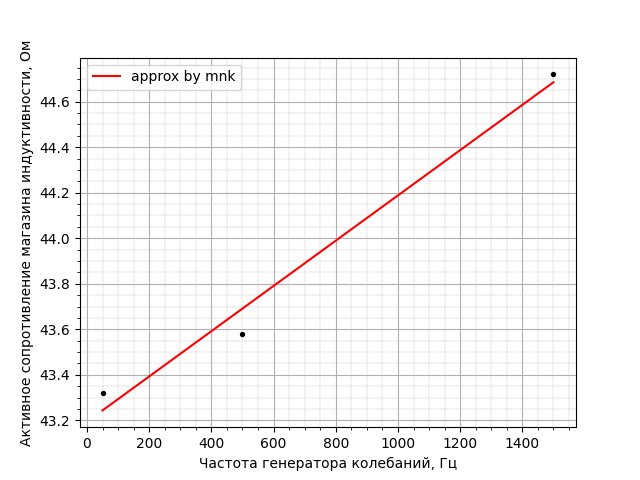
\includegraphics[width=15cm]{plot_2.png}
\end{center}
	\caption{\textit{График зависимости активного сопротивления катушки от частоты генератора колебаний}}
	\label{img1}
\end{figure}

\section{Вывод}

В данной лабораторной работе мы исследовали свободные и вынужденные колебания в электрическом контуре и различными способами находили его добротность.

\textbf{Итоговая таблица:}
	\begin{table}[h]
		\centering
		\begin{tabular}{|c|c|c|c|c|c|}
			\hline
			$R$, Ом & $f(L, C, R)$ & $f(\theta)$ & Фаз. спираль & АЧХ & ФЧХ \\ \hline
			451 & $9.038 \pm 0,024$ & $8.139 \pm 0.163$& $10.44 \pm 0.731$ & $9.81$ & $6.139$ \\ \hline
			2042 & $1.893 \pm 0,005$ & $2.798 \pm 0.056$ & $2.73 \pm 0.191$ & $---$ & $---$ \\ \hline
		\end{tabular}
	\end{table}

\newpage

\subsection{Приложение}

\begin{figure}[h]
    \begin{minipage}[h]{0.5\linewidth}
        \center{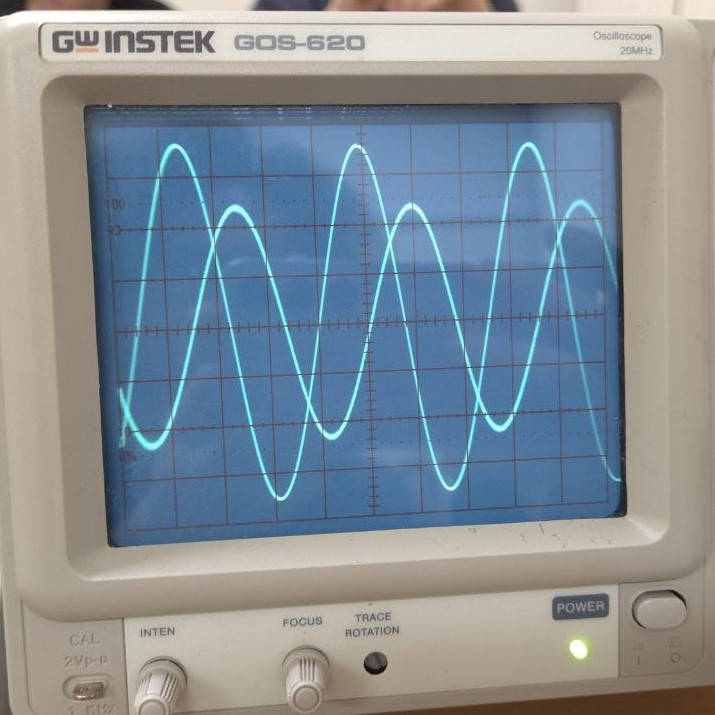
\includegraphics[width=0.8\linewidth]{1.jpg}}
    \end{minipage}
    \begin{minipage}[h]{0.5\linewidth}
        \center{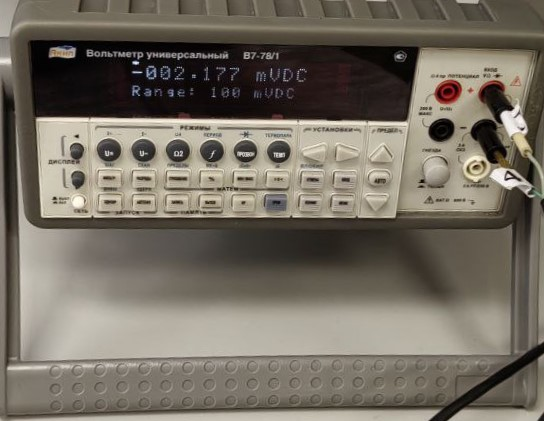
\includegraphics[width=0.8\linewidth]{2.jpg}}
    \end{minipage}
    \begin{minipage}[h]{0.5\linewidth}
        \center{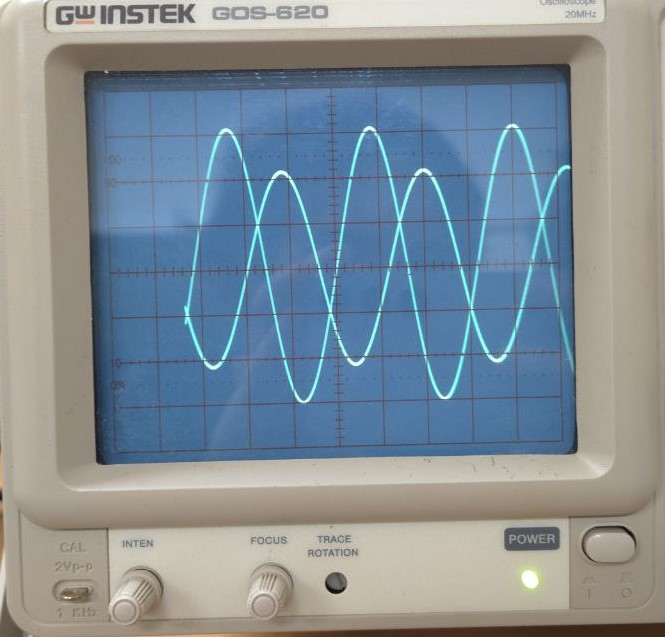
\includegraphics[width=0.8\linewidth]{3.jpg}}
    \end{minipage}
    \begin{minipage}[h]{0.5\linewidth}
        \center{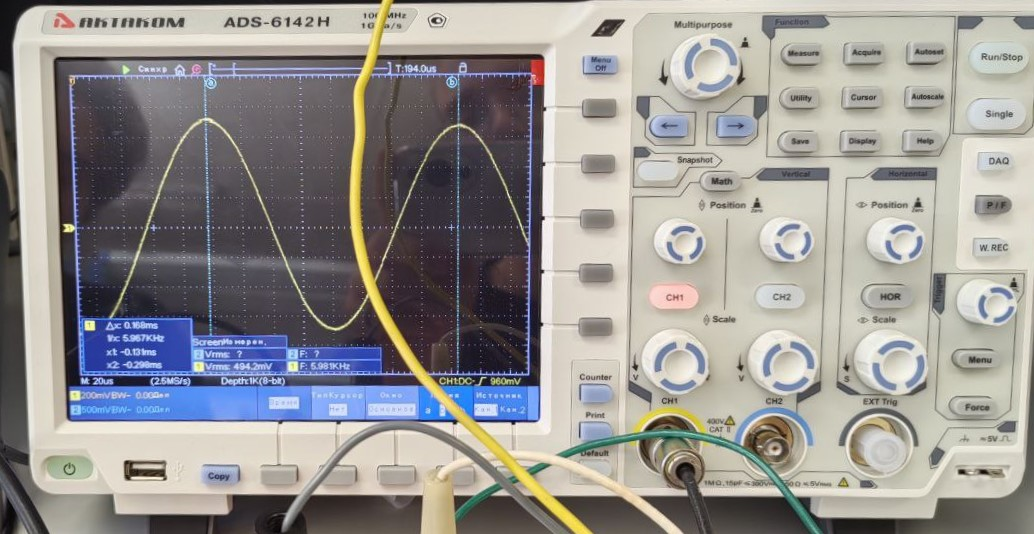
\includegraphics[width=0.8\linewidth]{4.jpg}}
    \end{minipage}
    \begin{minipage}[h]{0.5\linewidth}
        \center{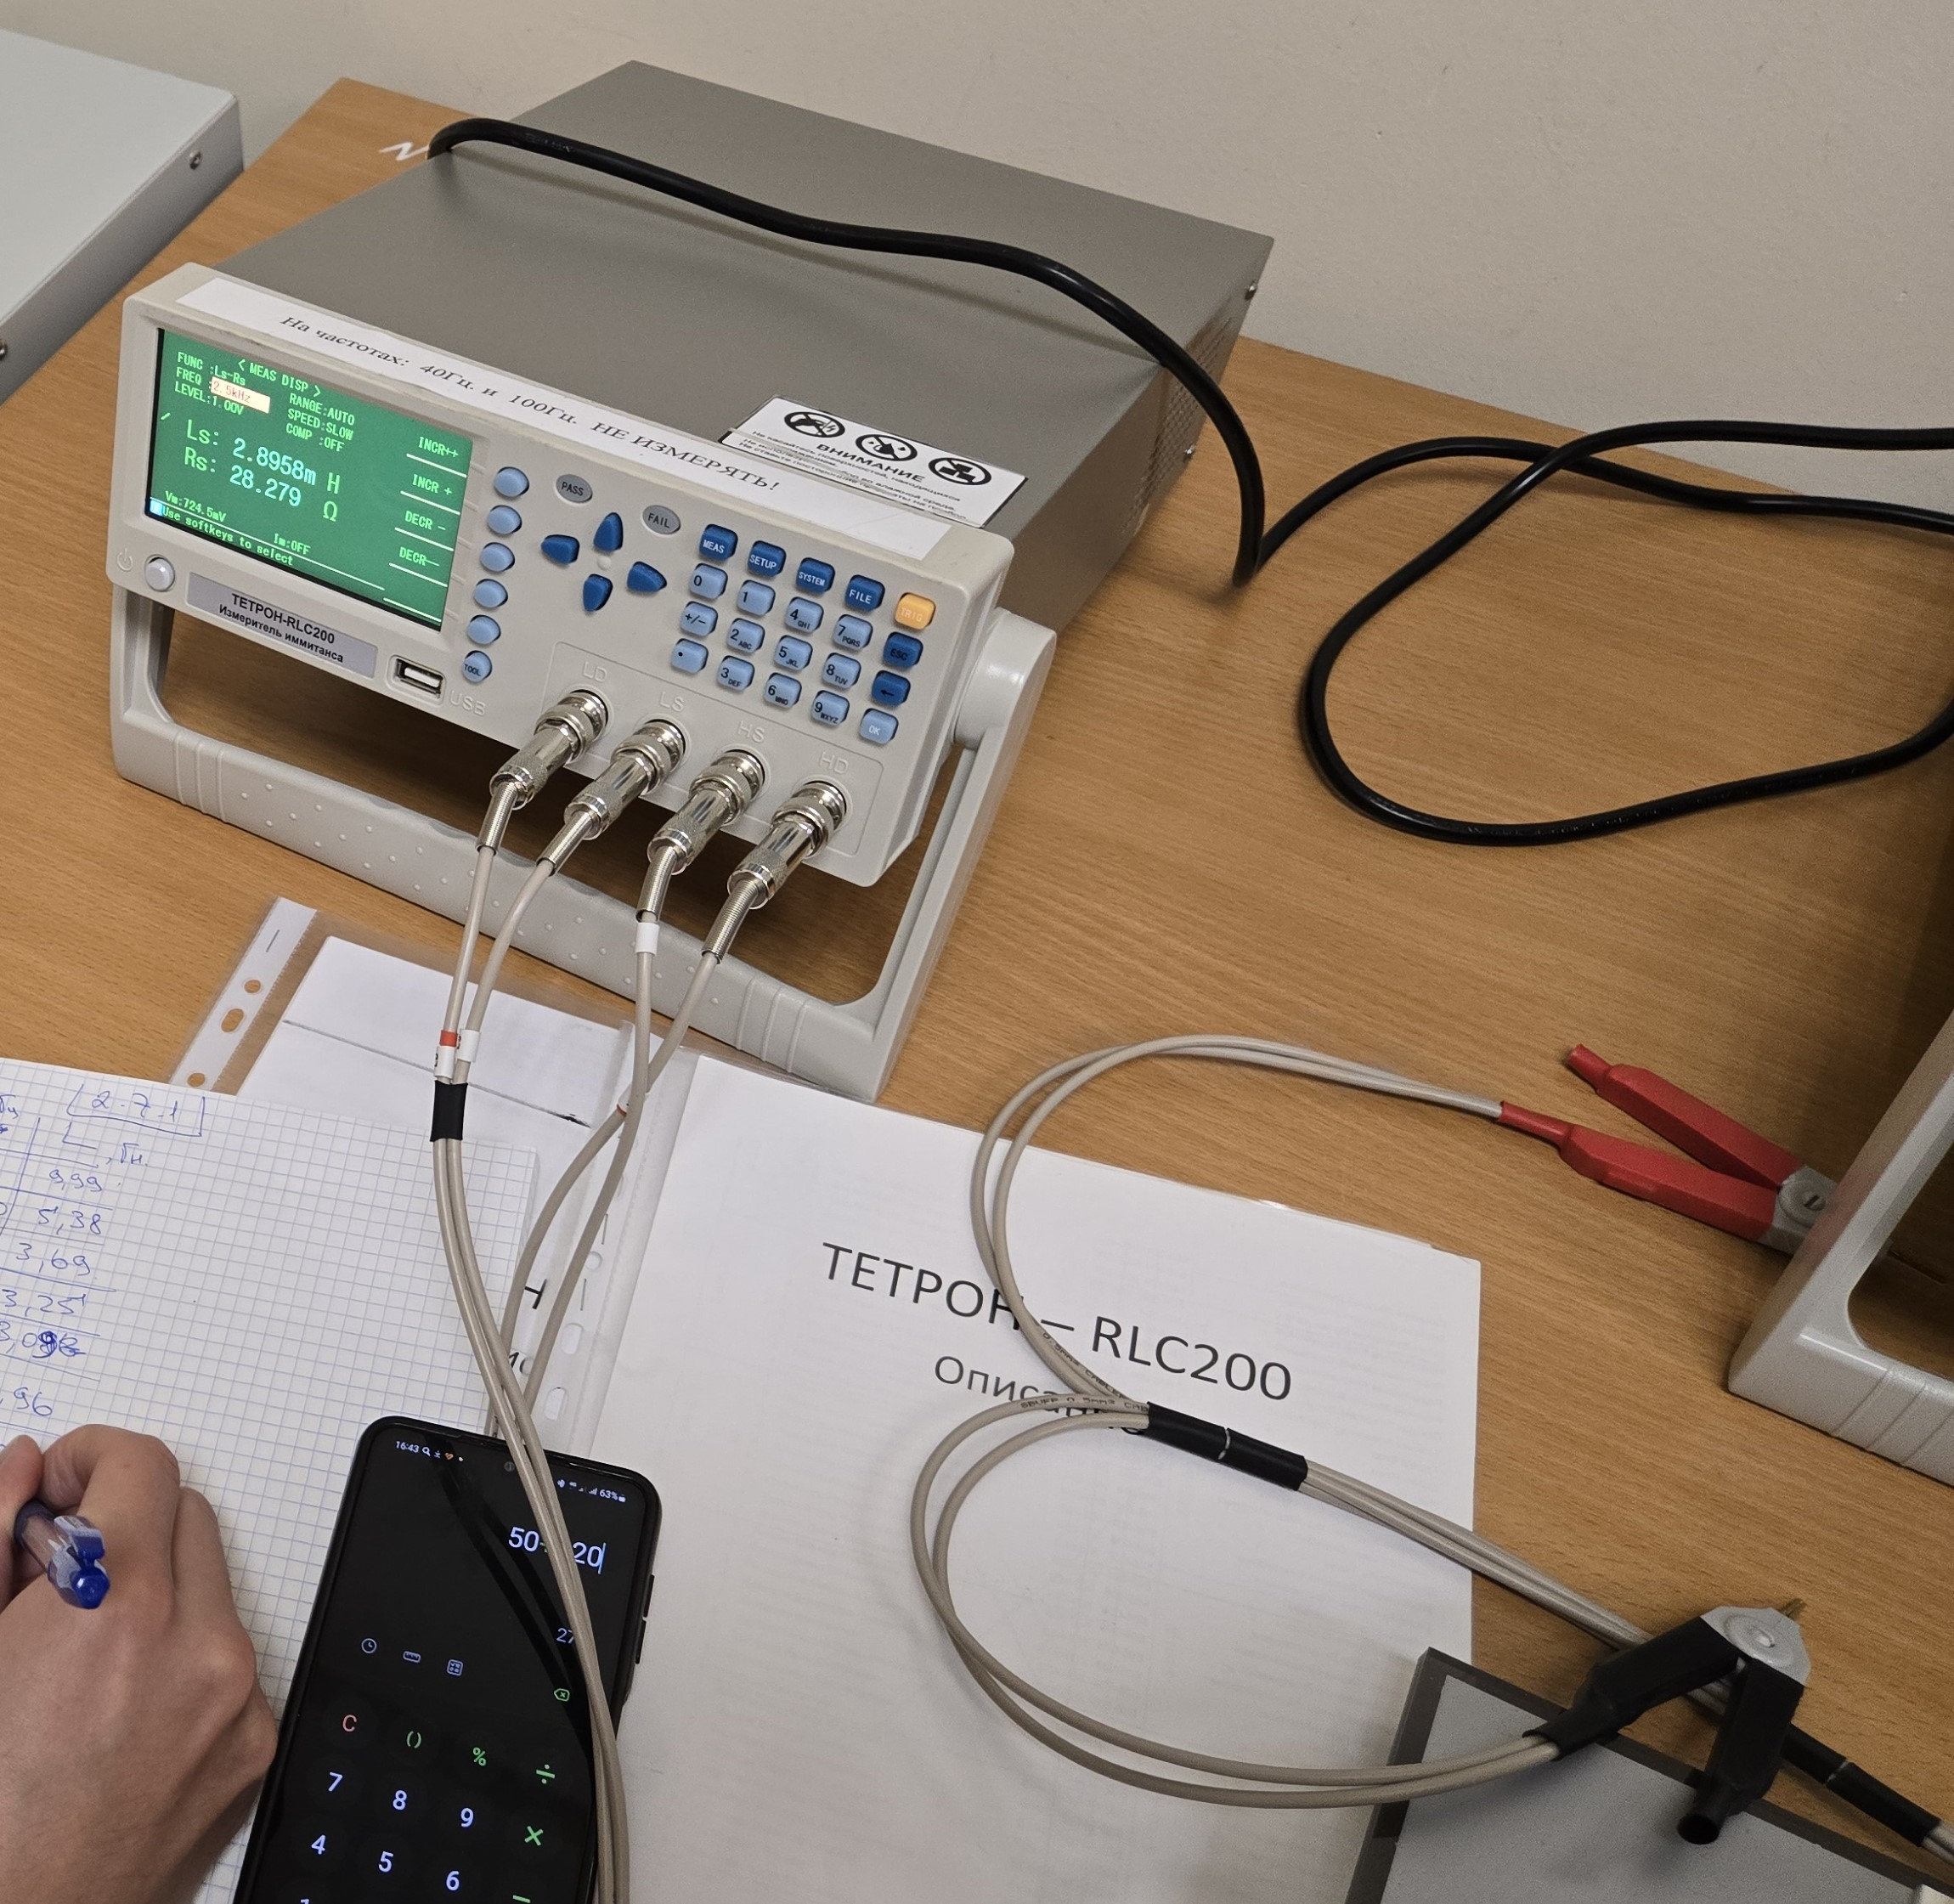
\includegraphics[width=0.8\linewidth]{5.jpg}}
    \end{minipage}
    \begin{minipage}[h]{0.5\linewidth}
        \center{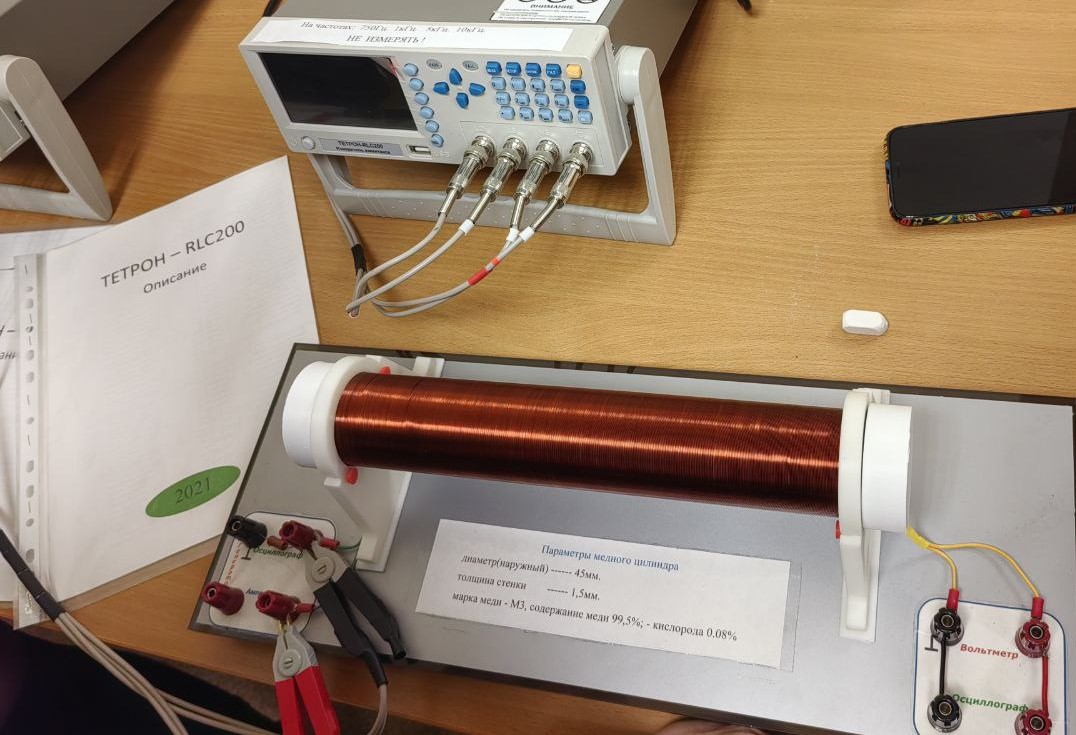
\includegraphics[width=0.8\linewidth]{6.jpg}}
    \end{minipage}
    \begin{minipage}[h]{0.5\linewidth}
        \center{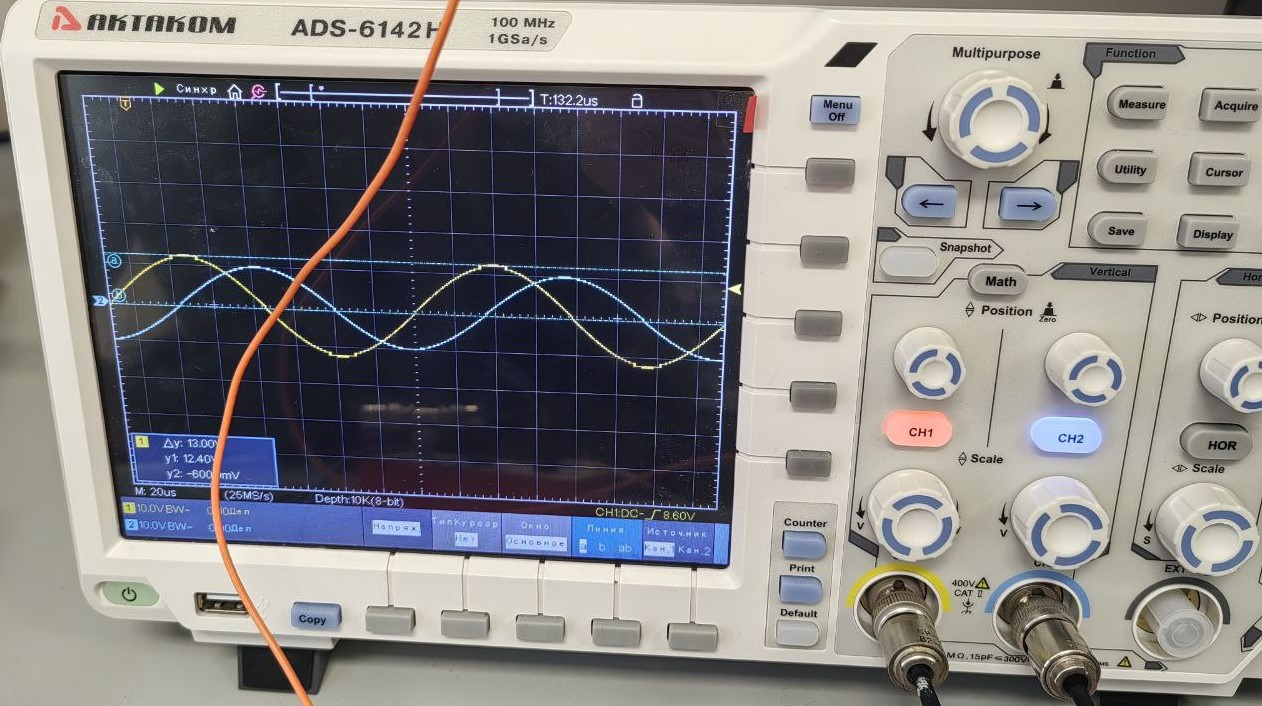
\includegraphics[width=0.8\linewidth]{9.jpg}}
    \end{minipage}
    \begin{minipage}[h]{0.5\linewidth}
        \center{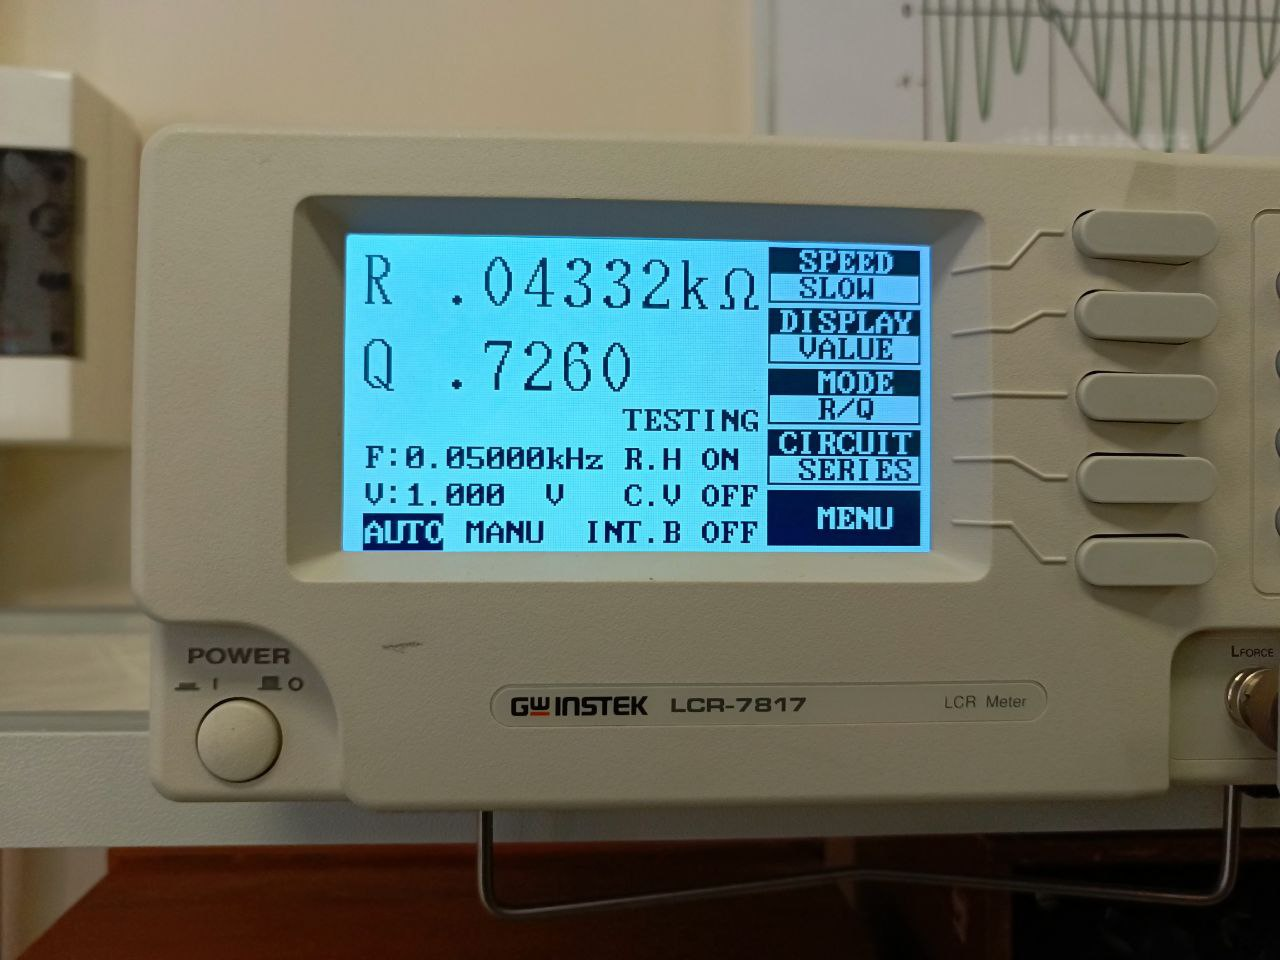
\includegraphics[width=0.7\linewidth]{8.png}}
    \end{minipage}
\end{figure}

\end{document}